%# -*- coding: utf-8 -*-
%!TEX encoding = UTF-8 Unicode
%!TEX TS-program = xelatex
% vim:ts=4:sw=4
%
% 以上设定默认使用 XeLaTex 编译,并指定 Unicode 编码,供 TeXShop 自动识别

% Author: Yunhui Fu <yhfudev@gmail.com>
% License: Creative Commons (CC BY 4.0)

\clearpage
\section{\cnt{Building Deep Networks for Classification}{建立分类用深度网络}{}}

\subsection{\cnt{From Self-Taught Learning to Deep Networks}{从自我学习到深层网络}{}}

\cnt{In the previous section(\ref{chp:selftaughtlearning}), you used an autoencoder to learn features that were then fed as input to a softmax or logistic regression classifier. In that method, the features were learned using only unlabeled data. In this section, we describe how you can \emph{fine-tune} and further improve the learned features using labeled data. When you have a large amount of labeled training data, this can significantly improve your classifier's performance. }
    {在前一节(\ref{chp:selftaughtlearning})中,我们利用自编码器来学习输入至 softmax 或 logistic 回归分类器的特征。这些特征仅利用未标注数据学习获得。在本节中,我们描述如何利用已标注数据进行\emph{微调},从而进一步优化这些特征。如果有大量已标注数据,通过微调就可以显著提升分类器的性能。 }
    {}


\cnt{In self-taught learning, we first trained a sparse autoencoder on the unlabeled data. Then, given a new example $x$, we used the hidden layer to extract features $a$. This is illustrated in the following diagram: }
    {在自我学习中,我们首先利用未标注数据训练一个稀疏自编码器。随后,给定一个新样本 $x$,我们通过隐含层提取出特征 $a$。上述过程图示如下: }
    {}

% duplicated figure:
\begin{figure}[ht] \centering
  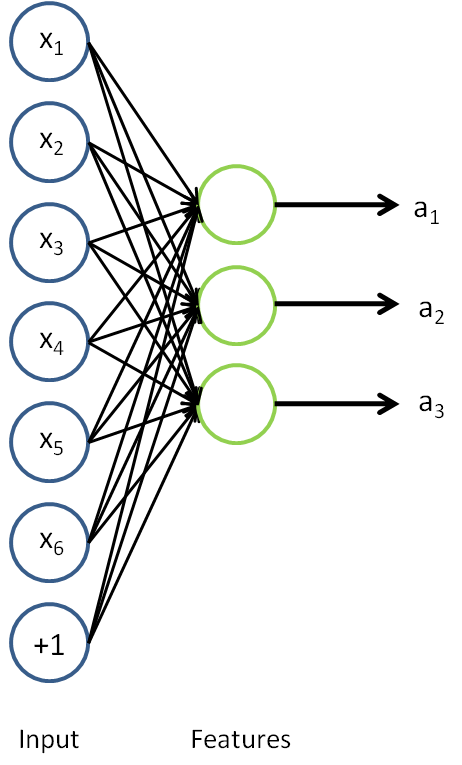
\includegraphics[width=0.4\textwidth]{figures/STL_SparseAE_Features.png}
  %\caption{}\label{fig:step1}
\end{figure}

\cnt{We are interested in solving a classification task, where our goal is to predict labels $y$. We have a labeled training set $\{ (x_l^{(1)}, y^{(1)}), (x_l^{(2)}, y^{(2)}), \ldots (x_l^{(m_l)}, y^{(m_l)}) \}$ of $m_l$ labeled examples. We showed previously that we can replace the original features $x^{(i)}$ with features $a^{(l)}$ computed by the sparse autoencoder (the ``replacement" representation). This gives us a training set $\{(a^{(1)}, y^{(1)}), \ldots (a^{(m_l)}, y^{(m_l)}) \}$. Finally, we train a logistic classifier to map from the features $a^{(i)}$ to the classification label $y^{(i)}$. To illustrate this step, similar to our earlier notes(\ref{chp:neuralnet}), we can draw our logistic regression unit (shown in orange) as follows: }
    {我们感兴趣的是分类问题,目标是预测样本的类别标号 $y$。我们拥有标注数据集 $\{ (x_l^{(1)}, y^{(1)}), (x_l^{(2)}, y^{(2)}), \ldots (x_l^{(m_l)},y^{(m_l)}) \}$,包含 $m_l$ 个标注样本。此前我们已经说明,可以利用稀疏自编码器获得的特征 $a^{(l)}$ 来替代原始特征。这样就可获得训练数据集 $\{(a^{(1)},y^{(1)}), \ldots (a^{(m_l)}, y^{(m_l)}) \}$。最终,我们训练出一个从特征 $a^{(i)}$ 到类标号 $y^{(i)}$ 的 logistic 分类器。为说明这一过程,我们按照神经网络一节(\ref{chp:neuralnet})中的方式,用下图描述 logistic 回归单元(橘黄色)。 }
    {}

\begin{figure}[ht] \centering
  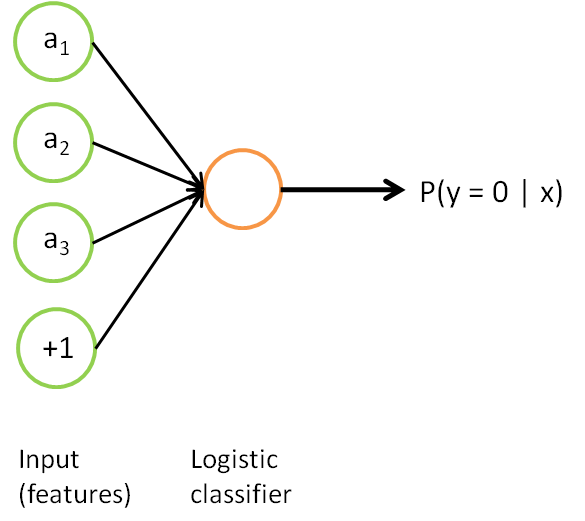
\includegraphics[width=0.5\textwidth]{figures/STL_Logistic_Classifier.png}
  %\caption{}\label{fig:step1}
\end{figure}

\cnt{Now, consider the overall classifier (i.e., the input-output mapping) that we have learned using this method. In particular, let us examine the function that our classifier uses to map from from a new test example $x$ to a new prediction $p(y = 1 | x)$. We can draw a representation of this function by putting together the two pictures from above. In particular, the final classifier looks like this:}
    {考虑利用这个方法所学到的分类器(输入-输出映射)。它描述了一个把测试样本 $x$ 映射到预测值 $p(y=1|x)$ 的函数。将此前的两张图片结合起来,就得到该函数的图形表示。也即,最终的分类器可以表示为: }
    {}

\begin{figure}[ht] \centering
  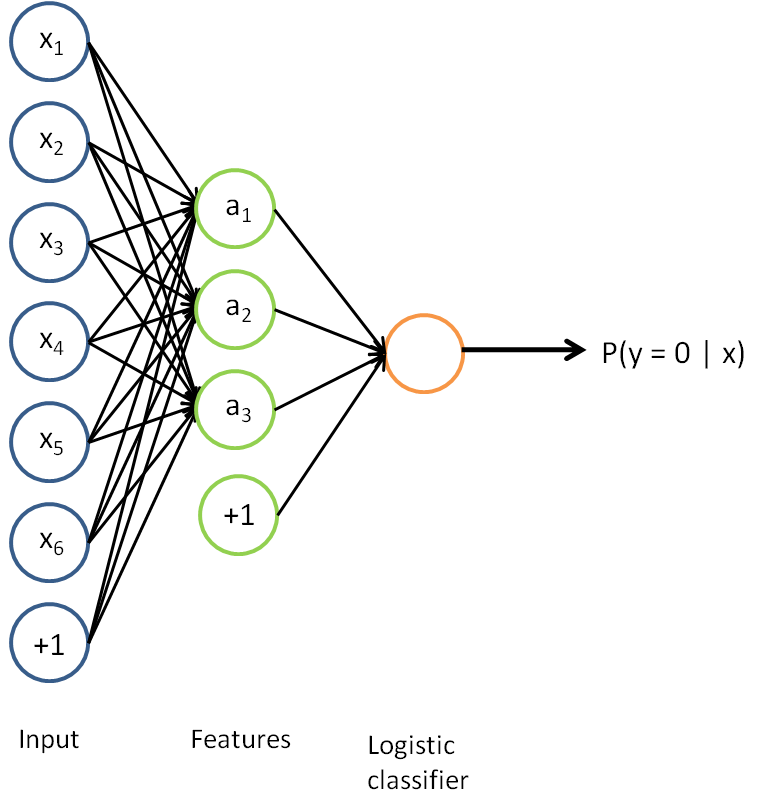
\includegraphics[width=0.57\textwidth]{figures/STL_CombinedAE.png}
  %\caption{}\label{fig:step1}
\end{figure}

\cnt{The parameters of this model were trained in two stages: The first layer of weights $W^{(1)}$ mapping from the input $x$ to the hidden unit activations $a$ were trained as part of the sparse autoencoder training process. The second layer of weights $W^{(2)}$ mapping from the activations $a$ to the output $y$ was trained using logistic regression (or softmax regression). }
    {该模型的参数通过两个步骤训练获得:在该网络的第一层,将输入 $x$ 映射至隐藏单元激活量 $a$ 的权值 $W^{(1)}$ 可以通过稀疏自编码器训练过程获得。在第二层,将隐藏单元 $a$ 映射至输出 $y$ 的权值 $W^{(2)}$ 可以通过 logistic 回归或 softmax 回归训练获得。}
    {}

\cnt{But the form of our overall/final classifier is clearly just a whole big neural network. So, having trained up an initial set of parameters for our model (training the first layer using an autoencoder, and the second layer via logistic/softmax regression), we can further modify all the parameters in our model to try to further reduce the training error. In particular, we can fine-tune the parameters, meaning perform gradient descent (or use L-BFGS) from the current setting of the parameters to try to reduce the training error on our labeled training set $\{ (x_l^{(1)}, y^{(1)}), (x_l^{(2)}, y^{(2)}), \ldots (x_l^{(m_l)}, y^{(m_l)}) \}$. }
    {这个最终分类器整体上显然是一个大的神经网络。因此,在训练获得模型最初参数(利用自动编码器训练第一层,利用 logistic/softmax 回归训练第二层)之后,我们可以进一步修正模型参数,进而降低训练误差。具体来说,我们可以对参数进行微调,在现有参数的基础上采用梯度下降或者 L-BFGS 来降低已标注样本集 $\{ (x_l^{(1)}, y^{(1)}), (x_l^{(2)}, y^{(2)}), \ldots (x_l^{(m_l)}, y^{(m_l)}) \}$ 上的训练误差。}
    {}

\cnt{When fine-tuning is used, sometimes the original unsupervised feature learning steps (i.e., training the autoencoder and the logistic classifier) are called \emph{pre-training}. The effect of fine-tuning is that the labeled data can be used to modify the weights $W^{(1)}$ as well, so that adjustments can be made to the features $a$ extracted by the layer of hidden units.}
    {使用微调时,初始的非监督特征学习步骤(也就是自动编码器和logistic分类器训练)有时候被称为\emph{预训练}。微调的作用在于,已标注数据集也可以用来修正权值 $W^{(1)}$,这样可以对隐藏单元所提取的特征 $a$ 做进一步调整。}
    {}

\cnt{So far, we have described this process assuming that you used the ``replacement" representation, where the training examples seen by the logistic classifier are of the form $(a^{(i)}, y^{(i)})$, rather than the ``concatenation" representation, where the examples are of the form $((x^{(i)}, a^{(i)}), y^{(i)})$. It is also possible to perform fine-tuning too using the ``concatenation" representation. (This corresponds to a neural network where the input units $x_i$ also feed directly to the logistic classifier in the output layer. You can draw this using a slightly different type of neural network diagram than the ones we have seen so far; in particular, you would have edges that go directly from the first layer input nodes to the third layer output node, ``skipping over" the hidden layer.) However, so long as we are using finetuning, usually the ``concatenation" representation has little advantage over the ``replacement" representation. Thus, if we are using fine-tuning usually we will do so with a network built using the replacement representation. (If you are not using fine-tuning however, then sometimes the concatenation representation can give much better performance.)}
    {到现在为止,我们描述上述过程时,都假设采用了“替代 (Replacement)”表示而不是“级联 (Concatenation)”表示。在替代表示中,logistic 分类器所看到的训练样本格式为 $(a^{(i)}, y^{(i)})$;而在级联表示中,分类器所看到的训练样本格式为 $((x^{(i)}, a^{(i)}), y^{(i)})$。对级联表示同样可以进行微调(在级联表示神经网络中,输入值 $x_i$ 也直接被输入至 logistic 分类器。对此前的神经网络示意图稍加更改,即可获得其示意图。具体的说,第一层的输入节点除了与隐层联接之外,还将越过隐层,与第三层输出节点直接相连)。但是对于微调来说,级联表示相对于替代表示几乎没有优势。因此,如果需要开展微调,我们通常使用替代表示的网络(但是如果不开展微调,级联表示的效果有时候会好得多)。}
    {}

\cnt{When should we use fine-tuning? It is typically used only if you have a large labeled training set; in this setting, fine-tuning can significantly improve the performance of your classifier. However, if you have a large \emph{unlabeled} dataset (for unsupervised feature learning/pre-training) and only a relatively small labeled training set, then fine-tuning is significantly less likely to help.}
    {在什么时候应用微调?通常仅在有大量已标注训练数据的情况下使用。在这样的情况下,微调能显著提升分类器性能。然而,如果有大量\emph{未标注}数据集(用于非监督特征学习/预训练),却只有相对较少的已标注训练集,微调的作用非常有限。}
    {}

\subsection{\cnt{Deep Networks: Overview}{深度网络概览}{}}


\subsubsection{\cnt{Overview}{概览}{}}

\cnt{In the previous sections, you constructed a 3-layer neural network comprising an input, hidden and output layer. While fairly effective for MNIST, this 3-layer model is a fairly \emph{shallow} network; by this, we mean that the features (hidden layer activations ${a}^{(2)}$) are computed using only ``one layer" of computation (the hidden layer).}
    {在之前的章节中,你已经构建了一个包括输入层、隐藏层以及输出层的三层神经网络。虽然该网络对于MNIST手写数字数据库非常有效,但是它还是一个非常“\emph{浅}”的网络。这里的“浅”指的是特征(隐藏层的激活值 ${a}^{(2)}$)只使用一层计算单元(隐藏层)来得到的。}
    {}

\cnt{In this section, we begin to discuss \emph{deep} neural networks, meaning ones in which we have multiple hidden layers; this will allow us to compute much more complex features of the input. Because each hidden layer computes a non-linear transformation of the previous layer, a deep network can have significantly greater representational power (i.e., can learn significantly more complex functions) than a shallow one.}
    {在本节中,我们开始讨论\emph{深度}神经网络,即含有多个隐藏层的神经网络。通过引入深度网络,我们可以计算更多复杂的输入特征。因为每一个隐藏层可以对上一层的输出进行非线性变换,因此深度神经网络拥有比“浅层”网络更加优异的表达能力(例如可以学习到更加复杂的函数关系)。}
    {}

\cnt{Note that when training a deep network, it is important to use a \emph{non-linear} activation function $f(\cdot)$ in each hidden layer. This is because multiple layers of linear functions would itself compute only a linear function of the input (i.e., composing multiple linear functions together results in just another linear function), and thus be no more expressive than using just a single layer of hidden units.}
    {值得注意的是当训练深度网络的时候,每一层隐层应该使用\emph{非线性}的激活函数 $f(\cdot)$。这是因为多层的线性函数组合在一起本质上也只有线性函数的表达能力(例如,将多个线性方程组合在一起仅仅产生另一个线性方程)。因此,在激活函数是线性的情况下,相比于单隐藏层神经网络,包含多隐藏层的深度网络并没有增加表达能力。}
    {}

\subsubsection{\cnt{Advantages of deep networks}{深度网络的优势}{}}

\cnt{Why do we want to use a deep network? The primary advantage is that it can compactly represent a significantly larger set of fuctions than shallow networks. Formally, one can show that there are functions which a $k$-layer network can represent compactly (with a number of hidden units that is \emph{polynomial} in the number of inputs), that a $(k - 1)$-layer network cannot represent unless it has an exponentially large number of hidden units.}
    {为什么我们要使用深度网络呢?使用深度网络最主要的优势在于,它能以更加紧凑简洁的方式来表达比浅层网络大得多的函数集合。正式点说,我们可以找到一些函数,这些函数可以用 $k$ 层网络简洁地表达出来(这里的简洁是指隐层单元的数目只需与输入单元数目呈\emph{多项式关系})。但是对于一个只有 $k-1$ 层的网络而言,除非它使用与输入单元数目呈指数关系的隐层单元数目,否则不能简洁表达这些函数。}
    {}

\cnt{To take a simple example, consider building a boolean circuit/network to compute the parity (or XOR) of $n$ input bits. Suppose each node in the network can compute either the logical OR of its inputs (or the OR of the negation of the inputs), or compute the logical AND. If we have a network with only one input, one hidden, and one output layer, the parity function would require a number of nodes that is exponential in the input size $n$. If however we are allowed a deeper network, then the network/circuit size can be only polynomial in n.}
    {举一个简单的例子,比如我们打算构建一个布尔网络来计算 $n$ 个输入比特的奇偶校验码(或者进行异或运算)。假设网络中的每一个节点都可以进行逻辑“或”运算(或者“与非”运算),亦或者逻辑“与”运算。如果我们拥有一个仅仅由一个输入层、一个隐层以及一个输出层构成的网络,那么该奇偶校验函数所需要的节点数目与输入层的规模 $n$ 呈指数关系。但是,如果我们构建一个更深点的网络,那么这个网络的规模就可做到仅仅是 $n$ 的多项式函数。}
    {}


\cnt{By using a deep network, in the case of images, one can also start to learn part-whole decompositions. For example, the first layer might learn to group together pixels in an image in order to detect edges (as seen in the earlier exercises). The second layer might then group together edges to detect longer contours, or perhaps detect simple ``parts of objects." An even deeper layer might then group together these contours or detect even more complex features.}
    {当处理对象是图像时,我们能够使用深度网络学习到“部分-整体”的分解关系。例如,第一层可以学习如何将图像中的像素组合在一起来检测边缘(正如我们在前面的练习中做的那样)。第二层可以将边缘组合起来检测更长的轮廓或者简单的“目标的部件”。在更深的层次上,可以将这些轮廓进一步组合起来以检测更为复杂的特征。}
    {}


\cnt{Finally, cortical computations (in the brain) also have multiple layers of processing. For example, visual images are processed in multiple stages by the brain, by cortical area ``V1", followed by cortical area ``V2" (a different part of the brain), and so on.}
    {最后要提的一点是,大脑皮层同样是分多层进行计算的。例如视觉图像在人脑中是分多个阶段进行处理的,首先是进入大脑皮层的“V1”区,然后紧跟着进入大脑皮层“V2”区,以此类推。}
    {}


\subsubsection{\cnt{Difficulty of training deep architectures}{训练深度网络的困难}{}}


\cnt{While the theoretical benefits of deep networks in terms of their compactness and expressive power have been appreciated for many decades, until recently researchers had little success training deep architectures.}
    {虽然几十年前人们就发现了深度网络在理论上的简洁性和较强的表达能力,但是直到最近,研究者们也没有在训练深度网络方面取得多少进步。}
    {}


\cnt{The main learning algorithm that researchers were using was to randomly initialize the weights of a deep network, and then train it using a labeled training set $\{ (x^{(1)}_l, y^{(1)}), \ldots, (x^{(m_l)}_l, y^{(m_l)}) \}$ using a supervised learning objective, for example by applying gradient descent to try to drive down the training error. However, this usually did not work well. There were several reasons for this.}
    {问题原因在于研究者们主要使用的学习算法是:首先随机初始化深度网络的权重,然后使用有监督的目标函数在有标签的训练集 $\left\{ \left( x_{l}^{\left( 1 \right)},{{y}^{\left( 1 \right)}} \right), \ldots, \left( x_{l}^{\left( {{m}_{l}} \right)},{{y}^{\left( {{m}_{l}} \right)}} \right) \right\}$ 上进行训练。例如通过使用梯度下降法来降低训练误差。然而,这种方法通常不是十分奏效。这其中有如下几方面原因:}
    {}



\textbf{\cnt{Availability of data}{数据获取问题}{}}


\cnt{With the method described above, one relies only on labeled data for training. However, labeled data is often scarce, and thus for many problems it is difficult to get enough examples to fit the parameters of a complex model. For example, given the high degree of expressive power of deep networks, training on insufficient data would also result in overfitting.}
    {使用上面提到的方法,我们需要依赖于有标签的数据才能进行训练。然而有标签的数据通常是稀缺的,因此对于许多问题,我们很难获得足够多的样本来拟合一个复杂模型的参数。例如,考虑到深度网络具有强大的表达能力,在不充足的数据上进行训练将会导致过拟合。}
    {}


\textbf{\cnt{Local optima}{局部极值问题}{}}


\cnt{Training a shallow network (with 1 hidden layer) using supervised learning usually resulted in the parameters converging to reasonable values; but when we are training a deep network, this works much less well. In particular, training a neural network using supervised learning involves solving a highly non-convex optimization problem (say, minimizing the training error $\sum_i ||h_W(x^{(i)}) - y^{(i)}||^2$ as a function of the network parameters $W$). In a deep network, this problem turns out to be rife with bad local optima, and training with gradient descent (or methods like conjugate gradient and L-BFGS) no longer work well.}
    {使用监督学习方法来对浅层网络(只有一个隐藏层)进行训练通常能够使参数收敛到合理的范围内。但是当用这种方法来训练深度网络的时候,并不能取得很好的效果。特别的,使用监督学习方法训练神经网络时,通常会涉及到求解一个高度非凸的优化问题(例如最小化训练误差 $\sum\nolimits_{i}{||{{h}_{W}}\left( {{x}^{\left( i \right)}} \right)-{{y}^{\left( i \right)}}|{{|}^{2}}}$,其中参数 $W$ 是要优化的参数。对深度网络而言,这种非凸优化问题的搜索区域中充斥着大量“坏”的局部极值,因而使用梯度下降法(或者像共轭梯度下降法,L-BFGS等方法)效果并不好。}
    {}


\textbf{\cnt{Diffusion of gradients}{梯度弥散问题}{}}

\cnt{There is an additional technical reason, pertaining to the gradients becoming very small, that explains why gradient descent (and related algorithms like L-BFGS) do not work well on a deep networks with randomly initialized weights. Specifically, when using backpropagation to compute the derivatives, the gradients that are propagated backwards (from the output layer to the earlier layers of the network) rapidly diminish in magnitude as the depth of the network increases. As a result, the derivative of the overall cost with respect to the weights in the earlier layers is very small. Thus, when using gradient descent, the weights of the earlier layers change slowly, and the earlier layers fail to learn much. This problem is often called the ``diffusion of gradients."}
    {梯度下降法(以及相关的L-BFGS算法等)在使用随机初始化权重的深度网络上效果不好的技术原因是:梯度会变得非常小。具体而言,当使用反向传播方法计算导数的时候,随着网络的深度的增加,反向传播的梯度(从输出层到网络的最初几层)的幅度值会急剧地减小。结果就造成了整体的损失函数相对于最初几层的权重的导数非常小。这样,当使用梯度下降法的时候,最初几层的权重变化非常缓慢,以至于它们不能够从样本中进行有效的学习。这种问题通常被称为“梯度的弥散”.}
    {}


\cnt{A closely related problem to the diffusion of gradients is that if the last few layers in a neural network have a large enough number of neurons, it may be possible for them to model the labeled data alone without the help of the earlier layers. Hence, training the entire network at once with all the layers randomly initialized ends up giving similar performance to training a shallow network (the last few layers) on corrupted input (the result of the processing done by the earlier layers).}
    {与梯度弥散问题紧密相关的问题是:当神经网络中的最后几层含有足够数量神经元的时候,可能单独这几层就足以对有标签数据进行建模,而不用最初几层的帮助。因此,对所有层都使用随机初始化的方法训练得到的整个网络的性能将会与训练得到的浅层网络(仅由深度网络的最后几层组成的浅层网络)的性能相似。}
    {}



\subsubsection{\cnt{Greedy layer-wise training}{逐层贪婪训练方法}{}}



\cnt{How can we train a deep network? One method that has seen some success is the \emph{greedy layer-wise training} method. We describe this method in detail in later sections, but briefly, the main idea is to train the layers of the network one at a time, so that we first train a network with 1 hidden layer, and only after that is done, train a network with 2 hidden layers, and so on. At each step, we take the old network with $k - 1$ hidden layers, and add an additional $k$-th hidden layer (that takes as input the previous hidden layer $k - 1$ that we had just trained). Training can either be supervised (say, with classification error as the objective function on each step), but more frequently it is unsupervised (as in an autoencoder; details to provided later). The weights from training the layers individually are then used to initialize the weights in the final/overall deep network, and only then is the entire architecture ``fine-tuned" (i.e., trained together to optimize the labeled training set error).}
    {那么,我们应该如何训练深度网络呢?\emph{逐层贪婪训练}方法是取得一定成功的一种方法。我们会在后面的章节中详细阐述这种方法的细节。简单来说,逐层贪婪算法的主要思路是每次只训练网络中的一层,即我们首先训练一个只含一个隐藏层的网络,仅当这层网络训练结束之后才开始训练一个有两个隐藏层的网络,以此类推。在每一步中,我们把已经训练好的前 $k-1$ 层固定,然后增加第 $k$ 层(也就是将我们已经训练好的前 $k-1$ 的输出作为输入)。每一层的训练可以是有监督的(例如,将每一步的分类误差作为目标函数),但更通常使用无监督方法(例如自动编码器,我们会在后边的章节中给出细节)。这些各层单独训练所得到的权重被用来初始化最终(或者说全部)的深度网络的权重,然后对整个网络进行“微调”(即把所有层放在一起来优化有标签训练集上的训练误差).}
    {}

\cnt{The success of greedy layer-wise training has been attributed to a number of factors:}
    {逐层贪婪的训练方法取得成功要归功于以下几方面:}
    {}

\textbf{\cnt{Availability of data}{数据获取}{}}


\cnt{While labeled data can be expensive to obtain, unlabeled data is cheap and plentiful. The promise of self-taught learning is that by exploiting the massive amount of unlabeled data, we can learn much better models. By using unlabeled data to learn a good initial value for the weights in all the layers $W^{(l)}$ (except for the final classification layer that maps to the outputs/predictions), our algorithm is able to learn and discover patterns from massively more amounts of data than purely supervised approaches. This often results in much better classifiers being learned.}
    {虽然获取有标签数据的代价是昂贵的,但获取大量的无标签数据是容易的。自学习方法(self-taught learning)的潜力在于它能通过使用大量的无标签数据来学习到更好的模型。具体而言,该方法使用无标签数据来学习得到所有层(不包括用于预测标签的最终分类层)${{W}^{(l)}}$ 的最佳初始权重。相比纯监督学习方法,这种自学习方法能够利用多得多的数据,并且能够学习和发现数据中存在的模式。因此该方法通常能够提高分类器的性能。}
    {}


\textbf{\cnt{Better local optima}{更好的局部极值}{}}

\cnt{After having trained the network on the unlabeled data, the weights are now starting at a better location in parameter space than if they had been randomly initialized. We can then further fine-tune the weights starting from this location. Empirically, it turns out that gradient descent from this location is much more likely to lead to a good local minimum, because the unlabeled data has already provided a significant amount of ``prior" information about what patterns there are in the input data.}
    {当用无标签数据训练完网络后,相比于随机初始化而言,各层初始权重会位于参数空间中较好的位置上。然后我们可以从这些位置出发进一步微调权重。从经验上来说,以这些位置为起点开始梯度下降更有可能收敛到比较好的局部极值点,这是因为无标签数据已经提供了大量输入数据中包含的模式的先验信息。}
    {}

\cnt{In the next section, we will describe the specific details of how to go about implementing greedy layer-wise training.}
    {在下一节中,我们将会具体阐述如何进行逐层贪婪训练。}
    {}


\subsection{\cnt{Stacked Autoencoders}{栈式自编码算法}{}}

\subsubsection{\cnt{Overview}{概述}{}}


\cnt{The greedy layerwise approach for pretraining a deep network works by training each layer in turn. In this page, you will find out how autoencoders can be ``stacked" in a greedy layerwise fashion for pretraining (initializing) the weights of a deep network.}
    {逐层贪婪训练法依次训练网络的每一层,进而预训练整个深度神经网络。在本节中,我们将会学习如何将自编码器“栈化”到逐层贪婪训练法中,从而预训练(或者说初始化)深度神经网络的权重。}
    {}


\cnt{A stacked autoencoder is a neural network consisting of multiple layers of sparse autoencoders in which the outputs of each layer is wired to the inputs of the successive layer. Formally, consider a stacked autoencoder with n layers. Using notation from the autoencoder section, let $W^{(k, 1)}, W^{(k, 2)}, b^{(k, 1)}, b^{(k, 2)}$ denote the parameters $W^{(1)}, W^{(2)}, b^{(1)}, b^{(2)}$ for kth autoencoder. Then the encoding step for the stacked autoencoder is given by running the encoding step of each layer in forward order:}
    {栈式自编码神经网络是一个由多层稀疏自编码器组成的神经网络,其前一层自编码器的输出作为其后一层自编码器的输入。对于一个 $n$ 层栈式自编码神经网络,我们沿用自编码器一章的各种符号,假定用 $W^{(k, 1)}, W^{(k, 2)}, b^{(k, 1)}, b^{(k, 2)}$ 表示第 $k$ 个自编码器对应的 $W^{(1)}, W^{(2)}, b^{(1)}, b^{(2)}$ 参数,那么该栈式自编码神经网络的编码过程就是,按照从前向后的顺序执行每一层自编码器的编码步骤:}
    {}

\begin{align} a^{(l)} = f(z^{(l)}) \\ z^{(l + 1)} = W^{(l, 1)}a^{(l)} + b^{(l, 1)} \end{align}

\cnt{The decoding step is given by running the decoding stack of each autoencoder in reverse order:}
    {同理,栈式神经网络的解码过程就是,按照从后向前的顺序执行每一层自编码器的解码步骤:}
    {}

\begin{align} a^{(n + l)} = f(z^{(n + l)}) \\ z^{(n + l + 1)} = W^{(n - l, 2)}a^{(n + l)} + b^{(n - l, 2)} \end{align}


\cnt{The information of interest is contained within $a^{(n)}$, which is the activation of the deepest layer of hidden units. This vector gives us a representation of the input in terms of higher-order features.}
    {其中,$a^{(n)}$ 是最深层隐藏单元的激活值,其包含了我们感兴趣的信息,这个向量也是对输入值的更高阶的表示。}
    {}


\cnt{The features from the stacked autoencoder can be used for classification problems by feeding $a^{(n)}$ to a softmax classifier.}
    {通过将 $a^{(n)}$ 作为softmax分类器的输入特征,可以将栈式自编码神经网络中学到的特征用于分类问题。}
    {}

\textbf{\cnt{Training}{训练}{}}


\cnt{A good way to obtain good parameters for a stacked autoencoder is to use greedy layer-wise training. To do this, first train the first layer on raw input to obtain parameters $W^{(1,1)}, W^{(1,2)}, b^{(1,1)}, b^{(1,2)}$. Use the first layer to transform the raw input into a vector consisting of activation of the hidden units, A. Train the second layer on this vector to obtain parameters $W^{(2,1)}, W^{(2,2)}, b^{(2,1)}, b^{(2,2)}$. Repeat for subsequent layers, using the output of each layer as input for the subsequent layer.}
    {一种比较好的获取栈式自编码神经网络参数的方法是采用逐层贪婪训练法进行训练。即先利用原始输入来训练网络的第一层,得到其参数 $W^{(1,1)}, W^{(1,2)}, b^{(1,1)}, b^{(1,2)}$;然后网络第一层将原始输入转化成为由隐藏单元激活值组成的向量(假设该向量为A),接着把A作为第二层的输入,继续训练得到第二层的参数 $W^{(2,1)}, W^{(2,2)}, b^{(2,1)}, b^{(2,2)}$;最后,对后面的各层同样采用的策略,即将前层的输出作为下一层输入的方式依次训练。}
    {}


\cnt{This method trains the parameters of each layer individually while freezing parameters for the remainder of the model. To produce better results, after this phase of training is complete, fine-tuning(Fine-tuning Stacked AEs \ref{chp:fintuningstkae}) using backpropagation can be used to improve the results by tuning the parameters of all layers are changed at the same time.}
    {对于上述训练方式,在训练每一层参数的时候,会固定其它各层参数保持不变。所以,如果想得到更好的结果,在上述预训练过程完成之后,可以通过反向传播算法同时调整所有层的参数以改善结果,这个过程一般被称作“微调(fine-tuning)”。
    实际上,使用逐层贪婪训练方法将参数训练到快要收敛时,应该使用微调(\ref{chp:fintuningstkae})。反之,如果直接在随机化的初始权重上使用微调,那么会得到不好的结果,因为参数会收敛到局部最优。}
    {}

\notes{
\cnt{If one is only interested in finetuning for the purposes of classification, the common practice is to then discard the ``decoding" layers of the stacked autoencoder and link the last hidden layer $a^{(n)}$ to the softmax classifier. The gradients from the (softmax) classification error will then be backpropagated into the encoding layers.}
    {如果你只对以分类为目的的微调感兴趣,那么惯用的做法是丢掉栈式自编码网络的“解码”层,直接把最后一个隐藏层的 $a^{(n)}$ 作为特征输入到softmax分类器进行分类,这样,分类器(softmax)的分类错误的梯度值就可以直接反向传播给编码层了。}
    {}
}

\textbf{\cnt{Concrete example}{具体实例}{}}


\cnt{To give a concrete example, suppose you wished to train a stacked autoencoder with 2 hidden layers for classification of MNIST digits, as you will be doing in the next exercise(\ref{chp:execdeepnetdigitclass}).}
    {让我们来看个具体的例子,假设你想要训练一个包含两个隐含层的栈式自编码网络,用来进行MNIST手写数字分类(这将会是你的下一个练习)。}
    {}


\cnt{First, you would train a sparse autoencoder on the raw inputs $x^{(k)}$ to learn primary features $h^{(1)(k)}$ on the raw input.}
    {首先,你需要用原始输入 $x^{(k)}$ 训练第一个自编码器,它能够学习得到原始输入的一阶特征表示 $h^{(1)(k)}$(如下图所示)。}
    {}

\begin{figure}[ht] \centering
  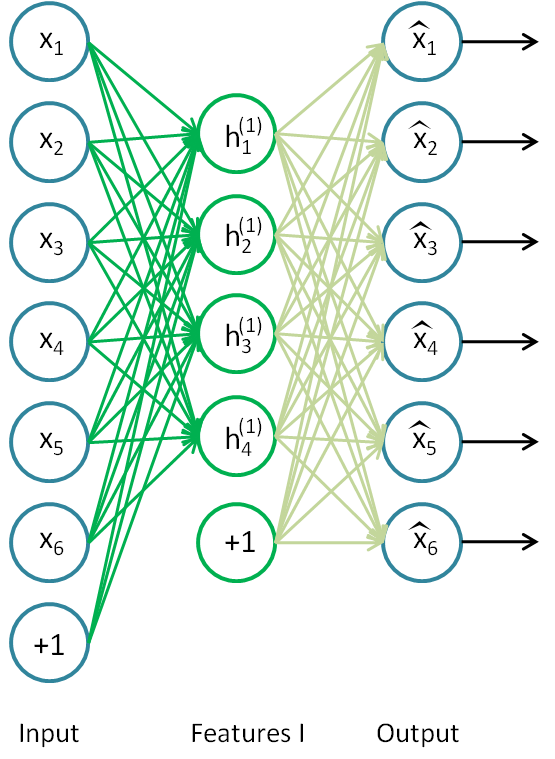
\includegraphics[width=0.5\textwidth]{figures/Stacked_SparseAE_Features1.png}
  %\caption{}\label{fig:step1}
\end{figure}


\cnt{Next, you would feed the raw input into this trained sparse autoencoder, obtaining the primary feature activations $h^{(1)(k)}$ for each of the inputs $x^{(k)}$. You would then use these primary features as the ``raw input" to another sparse autoencoder to learn secondary features $h^{(2)(k)}$ on these primary features.}
    {接着,你需要把原始数据输入到上述训练好的稀疏自编码器中,对于每一个输入 $x^{(k)}$,都可以得到它对应的一阶特征表示 $h^{(1)(k)}$。然后你再用这些一阶特征作为另一个稀疏自编码器的输入,使用它们来学习二阶特征 $h^{(2)(k)}$。(如下图所示)}
    {}


\begin{figure}[ht] \centering
  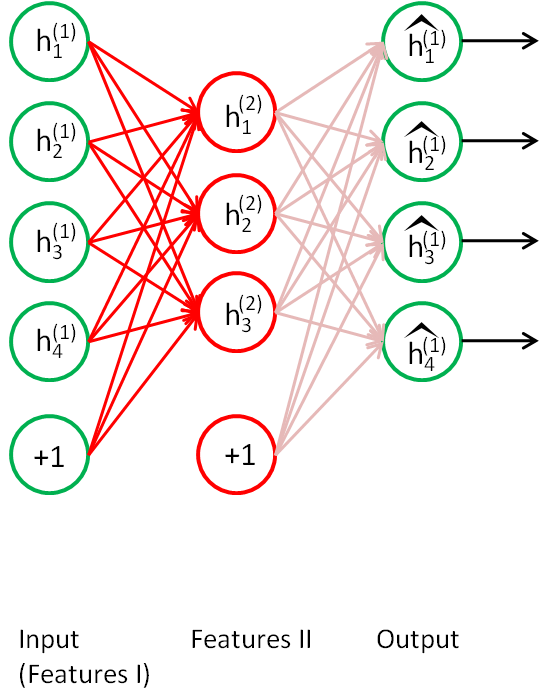
\includegraphics[width=0.5\textwidth]{figures/Stacked_SparseAE_Features2.png}
  %\caption{}\label{fig:step1}
\end{figure}

\cnt{Following this, you would feed the primary features into the second sparse autoencoder to obtain the secondary feature activations $h^{(2)(k)}$ for each of the primary features $h^{(1)(k)}$ (which correspond to the primary features of the corresponding inputs $x^{(k)}$). You would then treat these secondary features as ``raw input" to a softmax classifier, training it to map secondary features to digit labels.}
    {同样,再把一阶特征输入到刚训练好的第二层稀疏自编码器中,得到每个 $h^{(1)(k)}$ 对应的二阶特征激活值 $h^{(2)(k)}$。接下来,你可以把这些二阶特征作为softmax分类器的输入,训练得到一个能将二阶特征映射到数字标签的模型。}
    {}

\begin{figure}[ht] \centering
  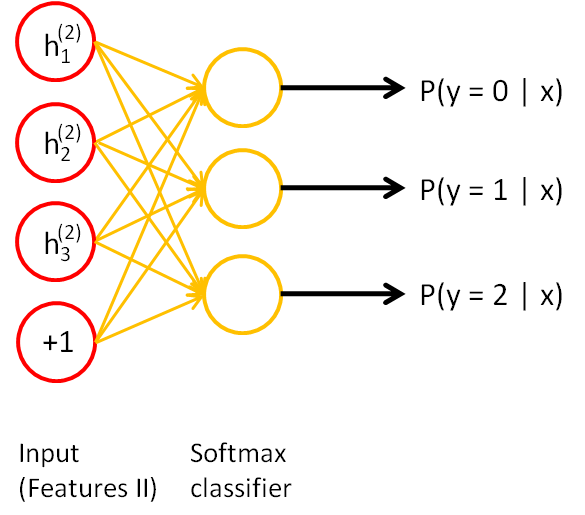
\includegraphics[width=0.5\textwidth]{figures/Stacked_Softmax_Classifier.png}
  %\caption{}\label{fig:step1}
\end{figure}

\cnt{Finally, you would combine all three layers together to form a stacked autoencoder with 2 hidden layers and a final softmax classifier layer capable of classifying the MNIST digits as desired.}
    {如下图所示,最终,你可以将这三层结合起来构建一个包含两个隐藏层和一个最终softmax分类器层的栈式自编码网络,这个网络能够如你所愿地对MNIST数字进行分类。}
    {}

\begin{figure}[ht] \centering
  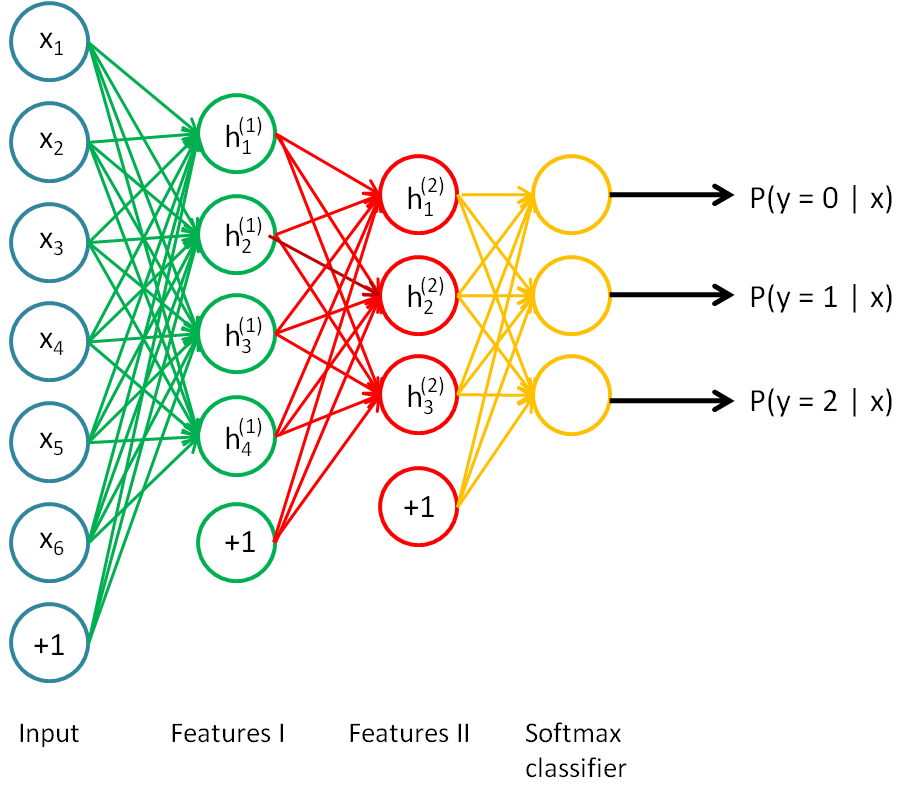
\includegraphics[width=0.5\textwidth]{figures/Stacked_Combined.png}
  %\caption{}\label{fig:step1}
\end{figure}

\textbf{\cnt{Discussion}{讨论}{}}


\cnt{A stacked autoencoder enjoys all the benefits of any deep network of greater expressive power.}
    {栈式自编码神经网络具有强大的表达能力及深度神经网络的所有优点。}
    {}


\cnt{Further, it often captures a useful ``hierarchical grouping" or ``part-whole decomposition" of the input. To see this, recall that an autoencoder tends to learn features that form a good representation of its input. The first layer of a stacked autoencoder tends to learn first-order features in the raw input (such as edges in an image). The second layer of a stacked autoencoder tends to learn second-order features corresponding to patterns in the appearance of first-order features (e.g., in terms of what edges tend to occur together--for example, to form contour or corner detectors). Higher layers of the stacked autoencoder tend to learn even higher-order features.}
    {更进一步,它通常能够获取到输入的“层次型分组”或者“部分-整体分解”结构。为了弄清这一点,回顾一下,自编码器倾向于学习得到能更好地表示输入数据的特征。因此,栈式自编码神经网络的第一层会学习得到原始输入的一阶特征(比如图片里的边缘),第二层会学习得到二阶特征,该特征对应一阶特征里包含的一些模式(比如在构成轮廓或者角点时,什么样的边缘会共现)。栈式自编码神经网络的更高层还会学到更高阶的特征。举个例子,如果网络的输入数据是图像,网络的第一层会学习如何去识别边,第二层一般会学习如何去组合边,从而构成轮廓、角等。更高层会学习如何去组合更形象且有意义的特征。例如,如果输入数据集包含人脸图像,更高层会学习如何识别或组合眼睛、鼻子、嘴等人脸器官。}
    {}


\subsection{\cnt{Fine-tuning Stacked AEs}{微调多层自编码算法}{}} \label{chp:fintuningstkae}


\subsubsection{\cnt{Introduction}{介绍}{}}

\cnt{Fine tuning is a strategy that is commonly found in deep learning. As such, it can also be used to greatly improve the performance of a stacked autoencoder. From a high level perspective, fine tuning treats all layers of a stacked autoencoder as a single model, so that in one iteration, we are improving upon all the weights in the stacked autoencoder.}
    {微调是深度学习中的常用策略,可以大幅提升一个栈式自编码神经网络的性能表现。从更高的视角来讲,微调将栈式自编码神经网络的所有层视为一个模型,这样在每次迭代中,网络中所有的权重值都可以被优化。}
    {}


\subsubsection{\cnt{General Strategy}{一般策略}{}}

\cnt{Fortunately, we already have all the tools necessary to implement fine tuning for stacked autoencoders! In order to compute the gradients for all the layers of the stacked autoencoder in each iteration, we use the Backpropagation Algorithm(\ref{chp:bkpropgationalg}), as discussed in the sparse autoencoder section. As the backpropagation algorithm can be extended to apply for an arbitrary number of layers, we can actually use this algorithm on a stacked autoencoder of arbitrary depth.}
    {幸运的是,实施微调栈式自编码神经网络所需的工具都已齐备!为了在每次迭代中计算所有层的梯度,我们需要使用稀疏自动编码一节中讨论的反向传播算法(\ref{chp:bkpropgationalg})。因为反向传播算法可以延伸应用到任意多层,所以事实上,该算法对任意多层的栈式自编码神经网络都适用。}
    {}


\subsubsection{\cnt{Finetuning with Backpropagation}{使用反向传播法进行微调}{}}

\cnt{For your convenience, the summary of the backpropagation algorithm using element wise notation is below:}
    {为方便读者,以下我们简要描述如何实施反向传播算法:}
    {}

\begin{enumerate}
  \item
    \cnt{Perform a feedforward pass, computing the activations for layers $L_2$, $L_3$, up to the output layer $L_{n_l}$, using the equations defining the forward propagation steps.}
      {进行一次前馈传递,对 $L_2$ 层、$L_3$ 层直到输出层 $L_{n_l}$,使用前向传播步骤中定义的公式计算各层上的激活值(激励响应)。}
      {}

  \item
    \cnt{For the output layer (layer $n_l$), set}
      {对输出层($n_l$ 层),令}
      {}

\begin{align} \delta^{(n_l)} = - (\nabla_{a^{n_l}}J) \bullet f'(z^{(n_l)}) \end{align} 
        \cnt{(When using softmax regression, the softmax layer has $\nabla J = \theta^T(I-P)$ where I is the input labels and P is the vector of conditional probabilities.)}
      {(当使用softmax分类器时,softmax层满足:$\nabla J = \theta^T(I-P)$,其中 $I$ 为输入数据对应的类别标签,$P$ 为条件概率向量。)}
      {}

  \item
    \cnt{For $l = n_l-1, n_l-2, n_l-3, \ldots, 2$; Set}
      {对 $l = n_l-1, n_l-2, n_l-3, \ldots, 2$; 令}
      {}

            \begin{align} \delta^{(l)} = \left((W^{(l)})^T \delta^{(l+1)}\right) \bullet f'(z^{(l)}) \end{align} 

  \item
    \cnt{Compute the desired partial derivatives:}
      {计算所需的偏导数:}
      {}

        \begin{align} \nabla_{W^{(l)}} J(W,b;x,y) &= \delta^{(l+1)} (a^{(l)})^T, \\ \nabla_{b^{(l)}} J(W,b;x,y) &= \delta^{(l+1)}. \end{align} 

    \begin{align} J(W,b) &= \left[ \frac{1}{m} \sum_{i=1}^m J(W,b;x^{(i)},y^{(i)}) \right] \end{align} 
\end{enumerate}

\cnt{Note: While one could consider the softmax classifier as an additional layer, the derivation above does not. Specifically, we consider the ``last layer" of the network to be the features that goes into the softmax classifier. Therefore, the derivatives (in Step 2) are computed using $\delta^{(n_l)} = - (\nabla_{a^{n_l}}J) \bullet f'(z^{(n_l)})$, where $\nabla J = \theta^T(I-P)$.}
    {注:我们可以认为输出层softmax分类器是附加上的一层,但是其求导过程需要单独处理。具体地说,网络“最后一层”的特征会进入softmax分类器。所以,第二步中的导数由 $\delta^{(n_l)} = - (\nabla_{a^{n_l}}J) \bullet f'(z^{(n_l)})$ 计算,其中 $\nabla J = \theta^T(I-P)$。}
    {}

\subsection{\cnt{Exercise: Implement deep networks for digit classification}{练习:实现数字分类的深度网络}{}} \label{chp:execdeepnetdigitclass}


\subsubsection{\cnt{Overview}{}{}}


\cnt{In this exercise, you will use a stacked autoencoder for digit classification. This exercise is very similar to the self-taught learning exercise, in which we trained a digit classifier using a autoencoder layer followed by a softmax layer. The only difference in this exercise is that we will be using two autoencoder layers instead of one and further finetune the two layers.}
    {}
    {}


\cnt{The code you have already implemented will allow you to stack various layers and perform layer-wise training. However, to perform fine-tuning, you will need to implement backpropogation through both layers. We will see that fine-tuning significantly improves the model's performance.}
    {}
    {}


\cnt{In the file \href{http://ufldl.stanford.edu/wiki/resources/stackedae_exercise.zip}{stackedae\_exercise.zip}, we have provided some starter code. You will need to complete the code in \texttt{stackedAECost.m}, \texttt{stackedAEPredict.m} and \texttt{stackedAEExercise.m}. We have also provided \texttt{params2stack.m} and \texttt{stack2params.m} which you might find helpful in constructing deep networks.}
    {}
    {}


\subsubsection{\cnt{Dependencies}{}{}}

\cnt{The following additional files are required for this exercise:}
    {}
    {}

\begin{itemize}
  \item MNIST Dataset \url{http://yann.lecun.com/exdb/mnist/}
  \item Support functions for loading MNIST in Matlab (\ref{chp:usemnistdata})
  \item Starter Code (\href{http://ufldl.stanford.edu/wiki/resources/stackedae_exercise.zip}{stackedae\_exercise.zip})
\end{itemize}


\cnt{You will also need your code from the following exercises:}
    {}
    {}
\begin{itemize}
  \item Exercise:Sparse Autoencoder (\ref{chp:execsparseautoenc})
  \item Exercise:Vectorization (\ref{chp:vecexec})
  \item Exercise:Softmax Regression (\ref{chp:execsoftmaxreg})
  \item Exercise:Self-Taught Learning (\ref{chp:execselftaughtlearn})
\end{itemize}

\emph{
\cnt{If you have not completed the exercises listed above, we strongly suggest you complete them first.}
    {}
    {}
}

\subsubsection{\cnt{Step 0: Initialize constants and parameters}{}{}}

\cnt{Open \texttt{stackedAEExercise.m}. In this step, we set meta-parameters to the same values that were used in previous exercise, which should produce reasonable results. You may to modify the meta-parameters if you wish.}
    {}
    {}


\subsubsection{\cnt{Step 1: Train the data on the first stacked autoencoder}{}{}}

\cnt{Train the first autoencoder on the training images to obtain its parameters. This step is identical to the corresponding step in the sparse autoencoder and STL assignments, complete this part of the code so as to learn a first layer of features using your \texttt{sparseAutoencoderCost.m} and \texttt{minFunc}.}
    {}
    {}


\subsubsection{\cnt{Step 2: Train the data on the second stacked autoencoder}{}{}}

\cnt{We first forward propagate the training set through the first autoencoder (using \texttt{feedForwardAutoencoder.m} that you completed in Exercise:Self-Taught Learning(\ref{chp:execselftaughtlearn}) ) to obtain hidden unit activations. These activations are then used to train the second sparse autoencoder. Since this is just an adapted application of a standard autoencoder, it should run similarly with the first. Complete this part of the code so as to learn a first layer of features using your \texttt{sparseAutoencoderCost.m} and \texttt{minFunc}.}
    {}
    {}

\cnt{This part of the exercise demonstrates the idea of greedy layerwise training with the same learning algorithm reapplied multiple times.}
    {}
    {}

\subsubsection{\cnt{Step 3: Train the softmax classifier on the L2 features}{}{}}

\cnt{Next, continue to forward propagate the L1 features through the second autoencoder (using \texttt{feedForwardAutoencoder.m}) to obtain the L2 hidden unit activations. These activations are then used to train the softmax classifier. You can either use \texttt{softmaxTrain.m} or directly use \texttt{softmaxCost.m} that you completed in Exercise:Softmax Regression(\ref{chp:execsoftmaxreg}) to complete this part of the assignment.}
    {}
    {}



\subsubsection{\cnt{Step 4: Implement fine-tuning}{}{}}

\cnt{To implement fine tuning, we need to consider all three layers as a single model. Implement \texttt{stackedAECost.m} to return the cost and gradient of the model. The cost function should be as defined as the log likelihood and a gradient decay term. The gradient should be computed using back-propagation as discussed earlier(\ref{chp:bkpropgationalg}). The predictions should consist of the activations of the output layer of the softmax model.}
    {}
    {}

\cnt{To help you check that your implementation is correct, you should also check your gradients on a synthetic small dataset. We have implemented \texttt{checkStackedAECost.m} to help you check your gradients. If this checks passes, you will have implemented fine-tuning correctly.}
    {}
    {}

\notes{
\cnt{\textbf{Note}: When adding the weight decay term to the cost, you should regularize only the softmax weights (do not regularize the weights that compute the hidden layer activations).}
    {}
    {}
}

\notes{
\cnt{\textbf{Implementation Tip}: It is always a good idea to implement the code modularly and check (the gradient of) each part of the code before writing the more complicated parts.}
    {}
    {}
}

\subsubsection{\cnt{Step 5: Test the model}{}{}}

\cnt{Finally, you will need to classify with this model; complete the code in \texttt{stackedAEPredict.m} to classify using the stacked autoencoder with a classification layer.}
    {}
    {}

\cnt{After completing these steps, running the entire script in stackedAETrain.m will perform layer-wise training of the stacked autoencoder, finetune the model, and measure its performance on the test set. If you've done all the steps correctly, you should get an accuracy of about 87.7\% before finetuning and 97.6\% after finetuning (for the 10-way classification problem).}
    {}
    {}

